
\subsection*{task 2.1 \\[1ex] (na\"ive) downsampling}

A rather simple idea for how to reduce the resolution of a digital (intensity) image is to keep only every $m$-th row and every $n$-th column of its pixels. For example, the figure below shows the effect of \emph{downsampling} by a factor of $2$, i.e. \emph{downsampling} by means of choosing $m = n = 2$.

Without using \keyword{for} loops, implement a function \keyword{downsample} with three parameters \texttt{arrF}, \texttt{m}, and \texttt{n} that realizes this manner of downsampling.

For $(m,n) \in \bigl\{ (4,4), (8,8) \bigr\}$, apply your method to image \texttt{portrait.png} and enter your results here
%%%%%
%%%%%
%%%%% enter your result here, i.e. replace "placeholder.pdf" by the names of your resulting image files
%%%%%
%%%%%
\begin{figure}[h!]
\subfloat[$256 \times 256$]{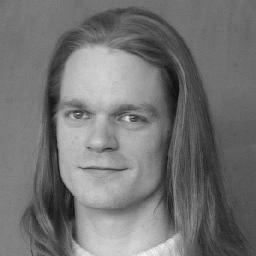
\includegraphics[width=0.40\textwidth]{portrait.png}} \hfill
\subfloat[$128 \times 128$]{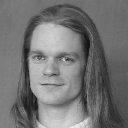
\includegraphics[width=0.20\textwidth]{t2-1-128x128.png}} \hfill
\subfloat[$64 \times 64$]{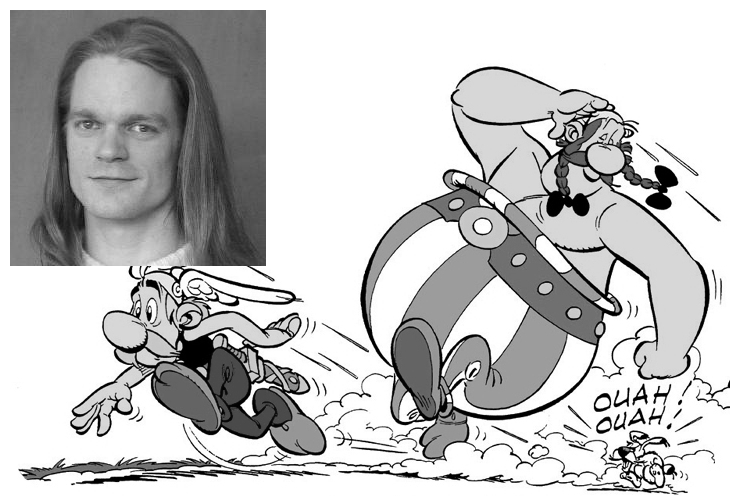
\includegraphics[width=0.10\textwidth]{t1-4.png}} \hfill
\subfloat[$32 \times 32$]{\makebox[1.5\width][c]{
\includegraphics[width=0.05\textwidth]{t1-8.png}}}
\end{figure}
%%%%%
%%%%%
%%%%%
%%%%%
%%%%%



\vspace{2cm}
Also, paste your code here 
%%%%%
%%%%%
%%%%% enter your code into the following environment
%%%%%
%%%%%
\begin{python}
def downsample(arrF, mn=(1, 1)):
    m, n = mn
    arrG = arrF[::m, ::n]
    return arrG
\end{python}
%%%%%
%%%%%
%%%%%
%%%%%
%%%%%
